\chapter{Benchmark}

Zur Durchf�hrung des Benchmarks wurde ein Transaktionsmix von sechs Queries und zugeh�riger Aufrufh�ufigkeit betrachtet:

\begin{itemize}
 
  \item Q1 - Sitzplatzverteilung Bundestag mit Kuchendiagramm (H�ufigkeit: 25\%)
  \item Q2 - Liste der Abgeordneten (H�ufigkeit: 10\%)
  \item Q3 - Detailergebnisse eines beliebigen Wahlkreises (H�ufigkeit: 25\%)
  \item Q4 - Wahlkreissieger mit eingef�rbter Deutschlandkarte (H�ufigkeit: 10\%)
  \item Q5 - �berhangsmandate (H�ufigkeit: 10\%)
  \item Q6 - Knappste Sieger und knappste Verlierer (H�ufigkeit: 20\%)
 
\end{itemize}

 Die Messung wurde mit 1, 2, 5, 7 und 10 parallel aktiven simulierten Browsern durchgef�hrt, die alle Queries 
 nach oben genannter H�ufigkeit in zuf�lliger Reihenfolge an einen lokalen Tomcat-Server stellten. 
 
 Auf dem Server lief Java-Code der die entsprechenden SQL-Statements an einen lokalen DB2-Server weiterleitete. Aus der DB2-Antwort wurde
 dann mittels Servlets eine HTML-Seite generiert und an den simulierten Browser gesendet, der die Zeit
 zwischen Anfrage und Antwort stoppte. Der Benchmark wurde auf einem Intel Core 2 Duo mit 1.50 GHz und 2.00 GB RAM durchgef�hrt. 
 
 \newpage
 
 Folgende Diagramme zeigen die Performance der einzelnen Quieres unter steigender Anzahl von parallelen Zugriffen.
 Auf der x-Achse befindet sich die Anzahl der parallel aktiven Browser und auf der
 y-Achse die dazugeh�rige durchschnittliche Server-Responsetime in Millisekunden. 
 
 Das Benchmark-Ergebnis mit einer Wartezeit von jeweils \emph{vier} Sekunden pro Browser zwischen den Queries:
 
 \begin{figure}[htbp]
	\centering
		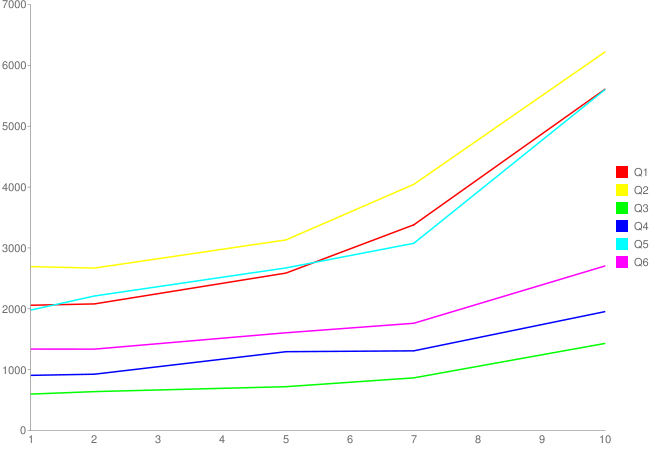
\includegraphics[width=0.85\textwidth]{figures/benchmark-4000.png}
	\caption{Durchschnittliche Response-Time bei einer Wartezeit von 4 Sekunden}
	\label{fig:benchmark-4000}
\end{figure}

 \newpage

 Das Benchmark-Ergebnis mit einer reduzierten Wartezeit von jeweils \emph{zwei} Sekunden pro Browser zwischen den Queries:
 
 \begin{figure}[htbp]
	\centering
		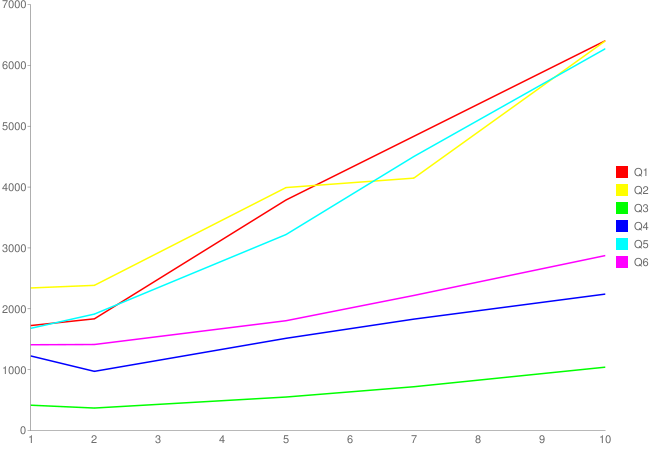
\includegraphics[width=0.85\textwidth]{figures/benchmark-2000.png}
	\caption{Durchschnittliche Response-Time bei einer Wartezeit von 2 Sekunden}
	\label{fig:benchmark-2000}
\end{figure}

